\section{Sample System Ouput - State Data}
This section contains the calculated states required to estimate a drag polar.
\begin{figure}[]
	\centering
	\caption{qbar vs. Time}
		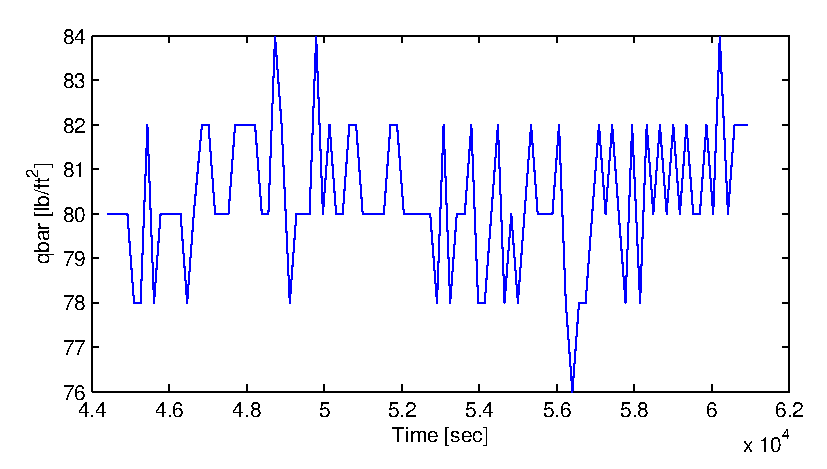
\includegraphics[width = 0.7\textwidth]{C:/Users/mufasa/Documents/Thesis/LaTex/figures/sampleOutput/State/qbar.eps}
\end{figure}
\begin{figure}[]
	\centering
	\caption{rho vs. Time}
		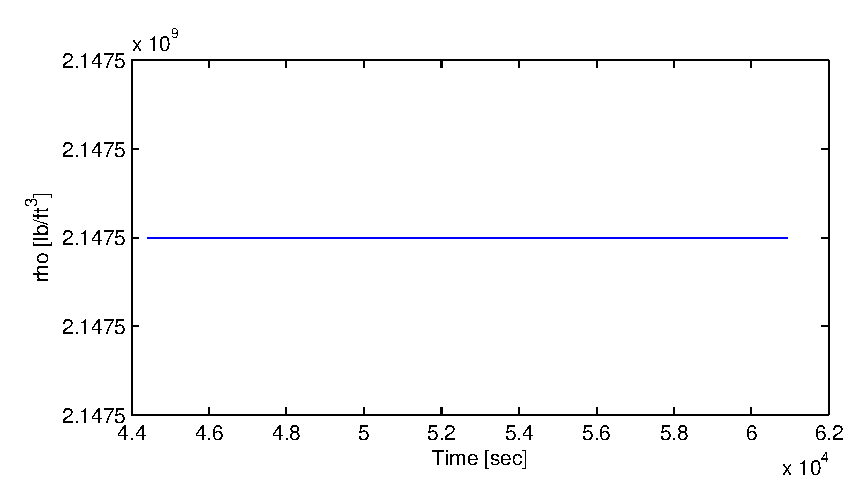
\includegraphics[width = 0.7\textwidth]{C:/Users/mufasa/Documents/Thesis/LaTex/figures/sampleOutput/State/rho.eps}
\end{figure}
\clearpage
\begin{figure}[]
	\centering
	\caption{alpha vs. Time}
		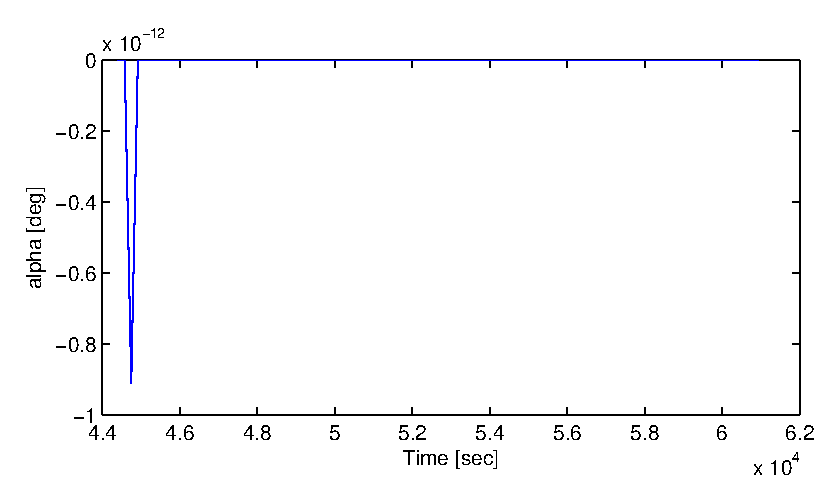
\includegraphics[width = 0.7\textwidth]{C:/Users/mufasa/Documents/Thesis/LaTex/figures/sampleOutput/State/alpha.eps}
\end{figure}
\begin{figure}[]
	\centering
	\caption{beta vs. Time}
		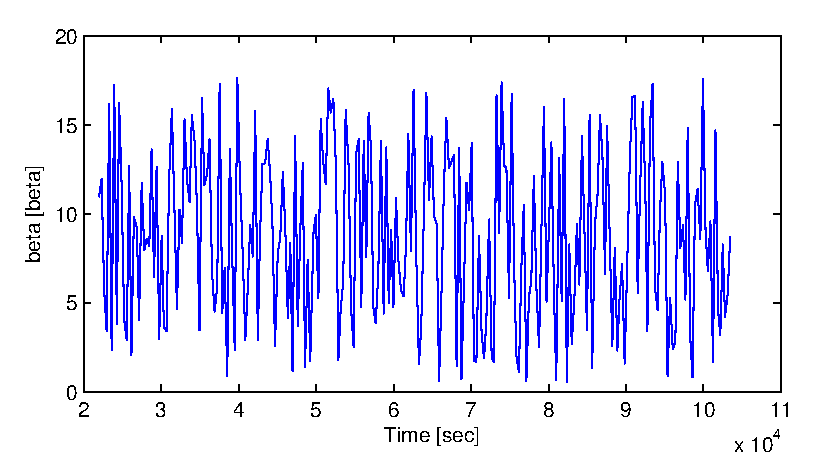
\includegraphics[width = 0.7\textwidth]{C:/Users/mufasa/Documents/Thesis/LaTex/figures/sampleOutput/State/beta.eps}
\end{figure}
\begin{figure}[]
	\centering
	\caption{roll vs. Time}
		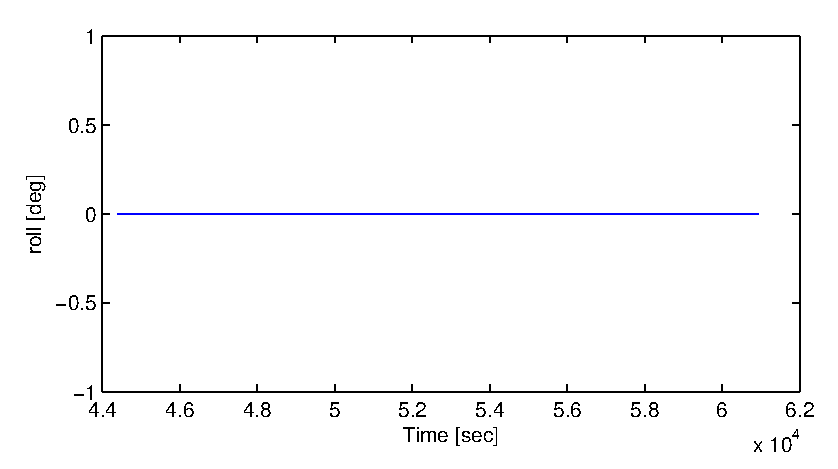
\includegraphics[width = 0.7\textwidth]{C:/Users/mufasa/Documents/Thesis/LaTex/figures/sampleOutput/State/roll.eps}
\end{figure}
\begin{figure}[]
	\centering
	\caption{pitch vs. Time}
		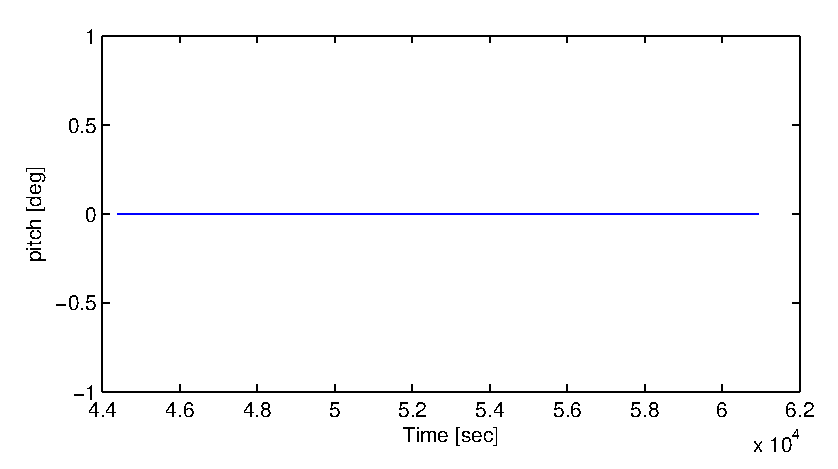
\includegraphics[width = 0.7\textwidth]{C:/Users/mufasa/Documents/Thesis/LaTex/figures/sampleOutput/State/pitch.eps}
\end{figure}
\begin{figure}[]
	\centering
	\caption{yaw vs. Time}
		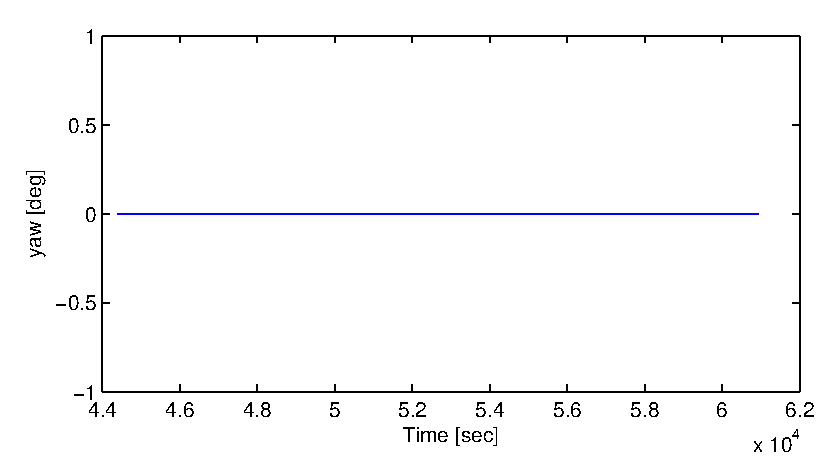
\includegraphics[width = 0.7\textwidth]{C:/Users/mufasa/Documents/Thesis/LaTex/figures/sampleOutput/State/yaw.eps}
\end{figure}
\begin{figure}[]
	\centering
	\caption{rollRate vs. Time}
		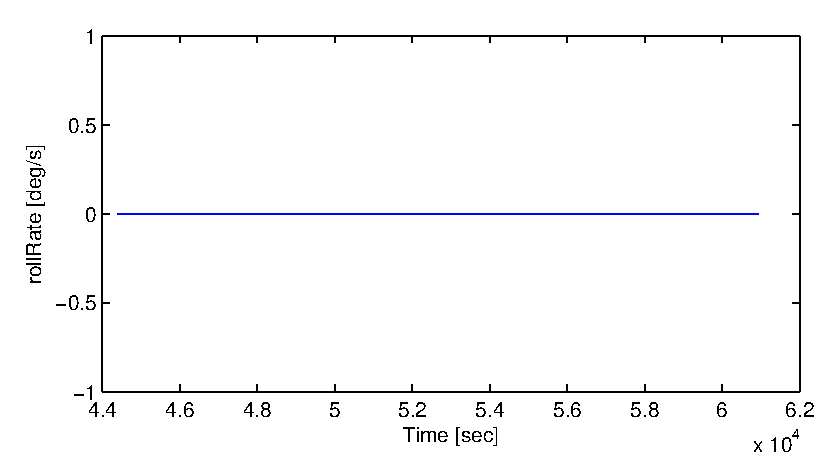
\includegraphics[width = 0.7\textwidth]{C:/Users/mufasa/Documents/Thesis/LaTex/figures/sampleOutput/State/rollRate.eps}
\end{figure}
\begin{figure}[]
	\centering
	\caption{pitchRate vs. Time}
		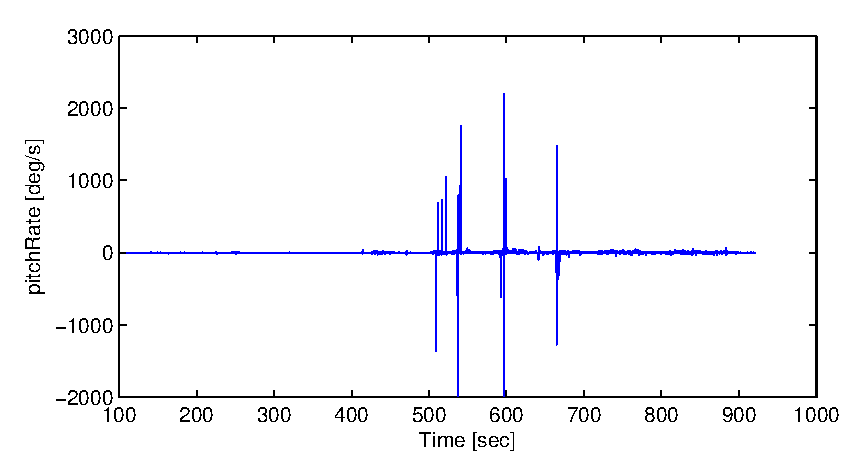
\includegraphics[width = 0.7\textwidth]{C:/Users/mufasa/Documents/Thesis/LaTex/figures/sampleOutput/State/pitchRate.eps}
\end{figure}
\begin{figure}[]
	\centering
	\caption{yawRate vs. Time}
		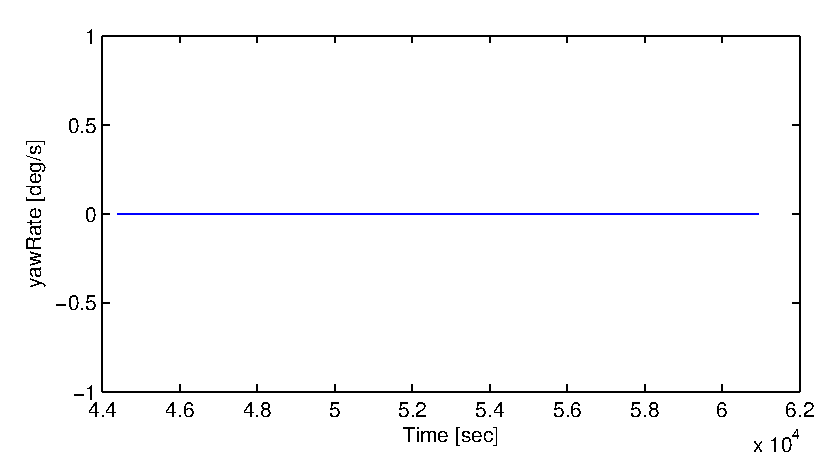
\includegraphics[width = 0.7\textwidth]{C:/Users/mufasa/Documents/Thesis/LaTex/figures/sampleOutput/State/yawRate.eps}
\end{figure}
\begin{figure}[]
	\centering
	\caption{accelX vs. Time}
		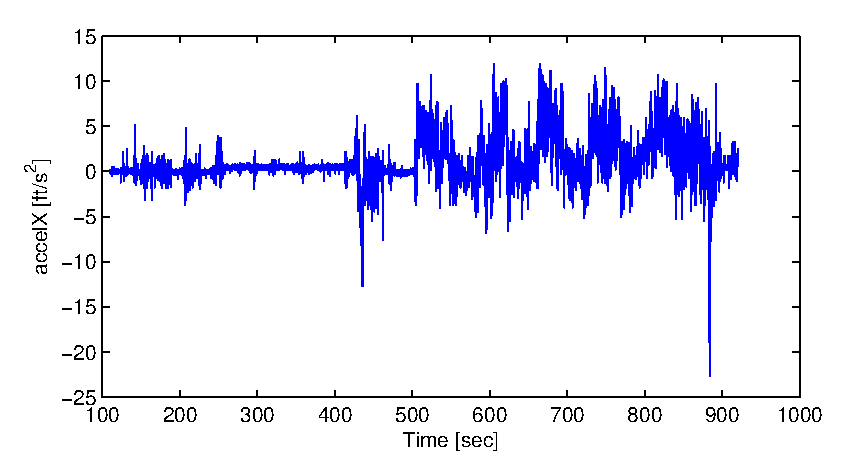
\includegraphics[width = 0.7\textwidth]{C:/Users/mufasa/Documents/Thesis/LaTex/figures/sampleOutput/State/accelX.eps}
\end{figure}
\begin{figure}[]
	\centering
	\caption{accelY vs. Time}
		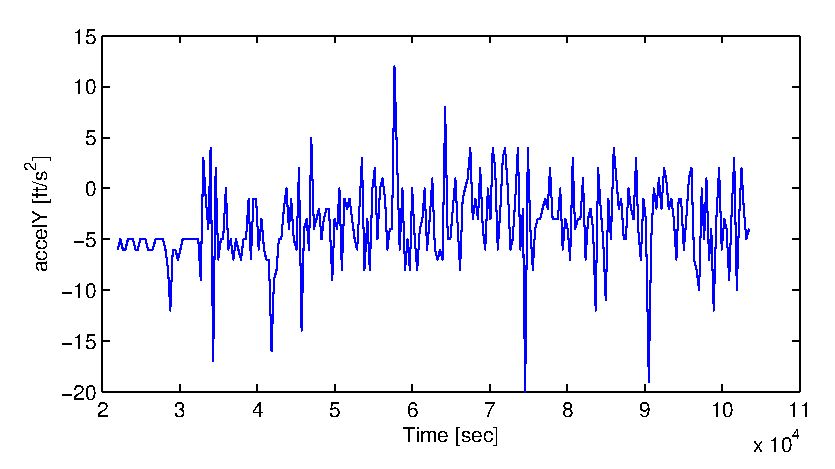
\includegraphics[width = 0.7\textwidth]{C:/Users/mufasa/Documents/Thesis/LaTex/figures/sampleOutput/State/accelY.eps}
\end{figure}
\begin{figure}[]
	\centering
	\caption{accelZ vs. Time}
		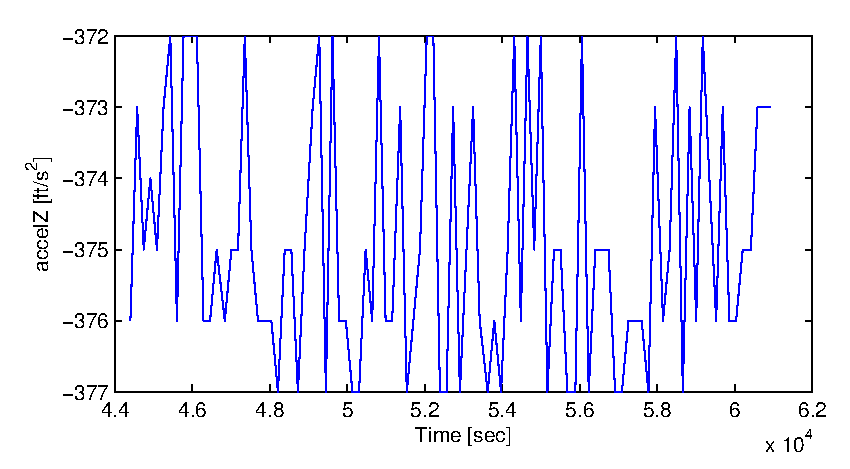
\includegraphics[width = 0.7\textwidth]{C:/Users/mufasa/Documents/Thesis/LaTex/figures/sampleOutput/State/accelZ.eps}
\end{figure}
